% BEGIN PREAMBEL
\documentclass[9pt]{beamer}
\usepackage[british]{babel}
%\usepackage{beamerarticle}
\usepackage[latin1]{inputenc}
\usepackage{amsmath,amsfonts,amssymb}
\usepackage{upgreek}
\newcommand{\as}{\\[14pt]}
\newcommand{\s}{\\[7pt]}
\newcommand{\is}{\\[2pt]}
\newcommand{\no}{\noindent}
\newcommand{\ka}{\hspace*{0.5cm}}
\newcommand{\ma}{\hspace*{1cm}}
\newcommand{\ga}{\hspace*{1.5cm}}
\newcommand{\li}{\left|}
\newcommand{\re}{\right|}
\newcommand{\const}{\text{const.}}
\newcommand{\z}{\text}
\newcommand{\terminal}[1]{\colorbox{black}{\textcolor{white}{{\fontfamily{phv}\selectfont \scriptsize{#1}}}}}
\newcommand{\plugin}[1]{\textit{\flq#1\frq}}
\usepackage{pgfpages}
\usepackage[version=3]{mhchem}
\usepackage{lmodern}
\usepackage{graphicx}
\usepackage{multicol}
\usepackage{xcolor}
\usepackage{wrapfig}
% \usepackage{uarial}
\usetheme{Boadilla}
\usecolortheme{beaver}
%\useinnertheme{circles}
\useoutertheme{miniframes}
%\setbeamercovered{transparent}
\beamertemplatenavigationsymbolsempty
%\setbeamertemplate{footline}[frame number]
\makeindex
\title[Master Thesis (Status)]{Status of the master thesis}
\author[M. Reichmann]{Michael Reichmann}
\institute[\textbf{\textit{ETH}}\scalebox{.6}{\textit{Z\"{u}rich}}]{Swiss Federal Institute of Technology Zurich / Low Energy Particle Physics}
% END PREAMBEL

% ============================
% START
% ============================
\begin{document}
% ============================
% TITLE PAGE
% ============================
\begin{frame}
	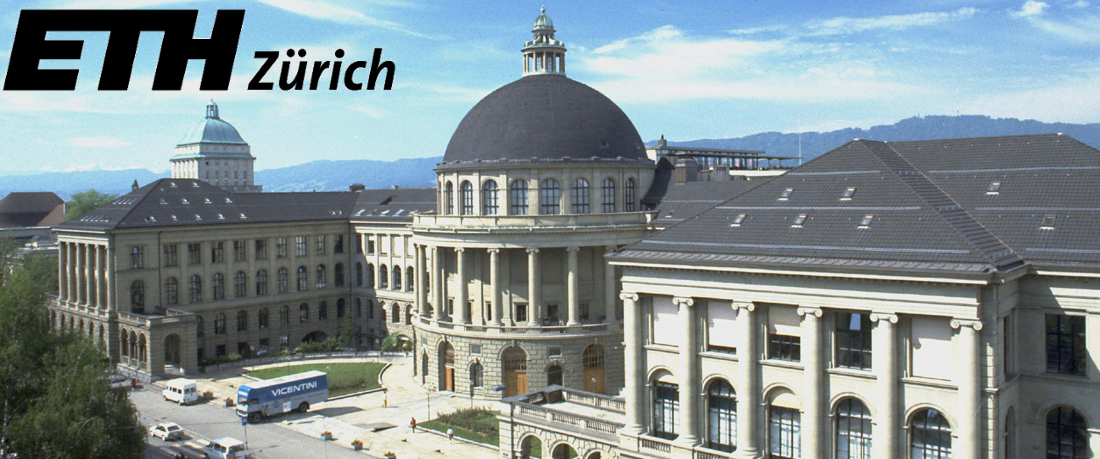
\includegraphics[width=\linewidth]{Pics/ETH-Zuerich}
	\vspace*{.7cm}
	\begin{alertblock}{
		\begin{center}
			\textbf{Status of my Master Thesis}
		\end{center}}
		\vspace*{10pt}
		\begin{center}\small
		Michael Reichmann
		\end{center}\normalsize
	\end{alertblock}
\end{frame}
% ============================
% TABLE OF CONTENTS
% ============================
\begin{frame}[allowframebreaks]
	\frametitle{Table of contents}
	\tableofcontents   % [pausesections]
\end{frame}

% ====================================================================================
% HARDWARE
% ====================================================================================
\section{Hardware}
% ============================
% THE PIXEL DETECTOR
% ============================
\subsection{The Silicon Pixel Detector}
\begin{frame}
	\frametitle{The Silicon Pixel Detector}
	\begin{itemize}
		\item silicon sensor electrically connected to a read out chip (ROC) via Indium bump bonds
		\item each silicon pixel connected to pixel unit cell (PUC) on the ROC
		\item $4160$ pixels in $26$ double columns and $80$ rows
		\item size of a pixel: $150\,\upmu$m $\times$ $100\,\upmu$m
		\item size of the sensor: $7.8\,$mm $\times$ $8.0\,$mm (area: $62.4\,$mm$^{2}$) 
	\end{itemize}
	\begin{center}
		\begin{minipage}{5cm}
			\centering
			\begin{figure}
				\caption{dimensions of the ROC in mm}
				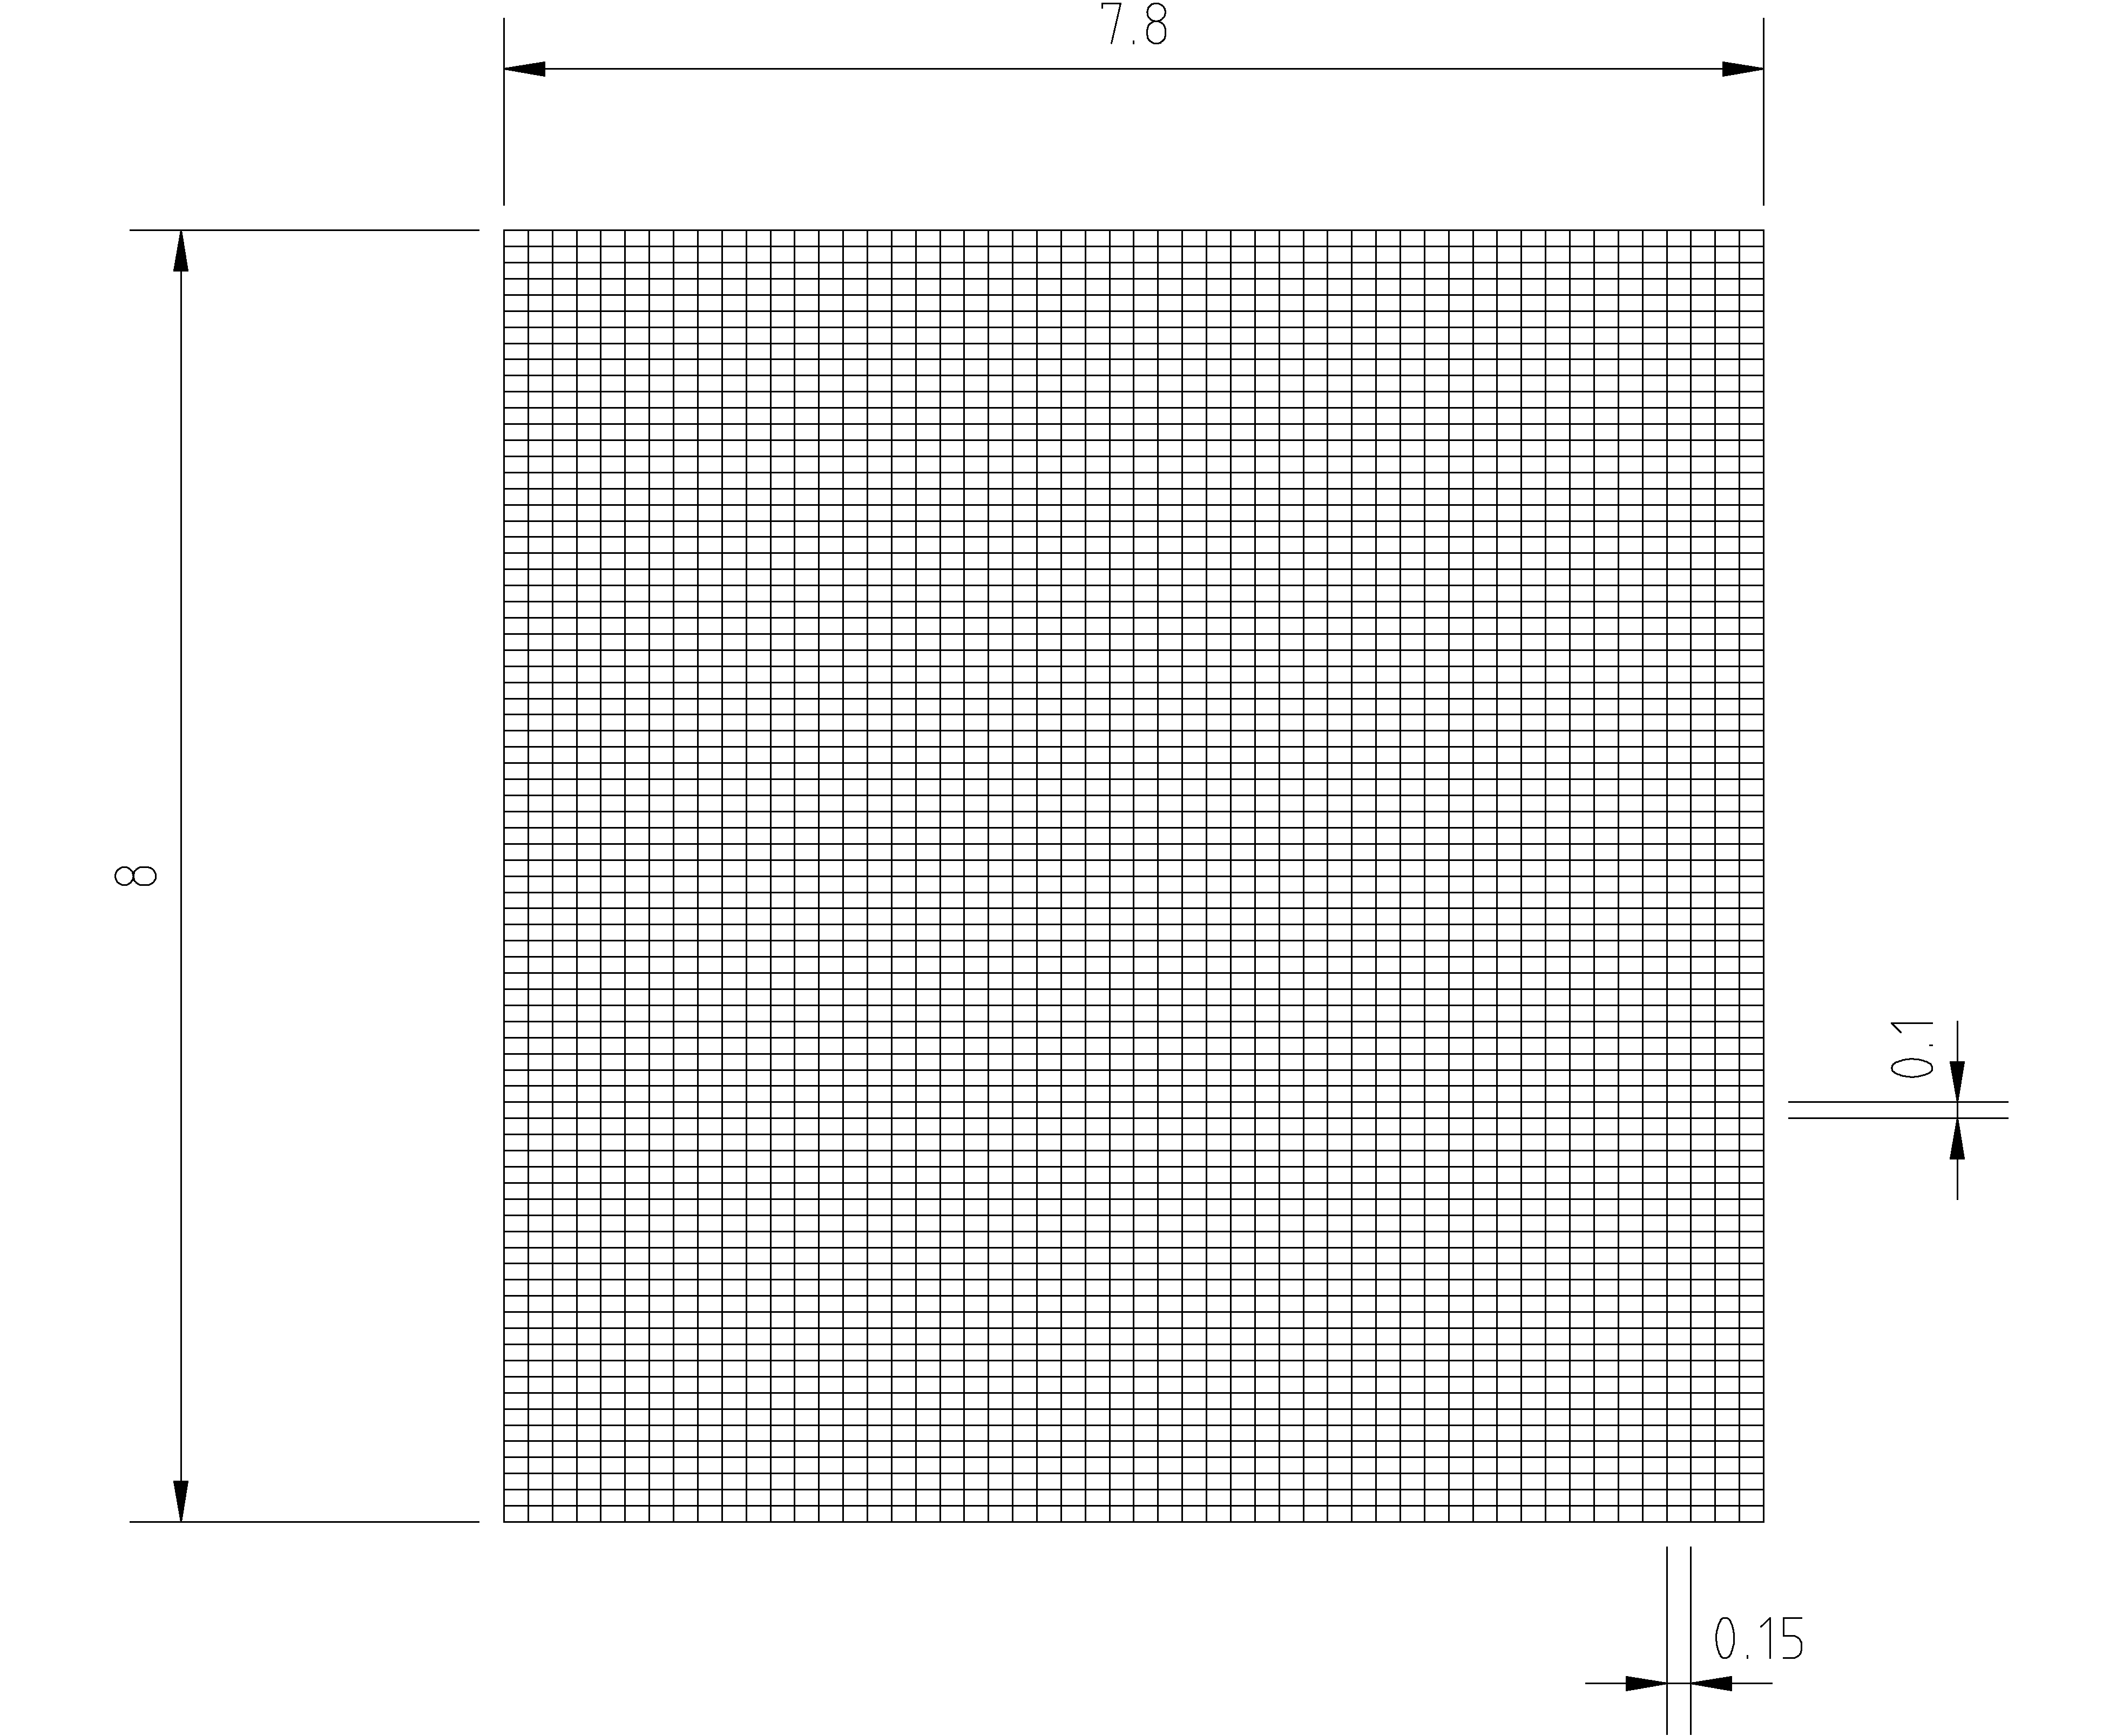
\includegraphics[height=3cm]{Pics/ROC1}
			\end{figure}
		\end{minipage}
		\hspace*{2pt}
		\begin{minipage}{5cm}
			\centering
			\begin{figure}
				\caption{analogue ROC}
				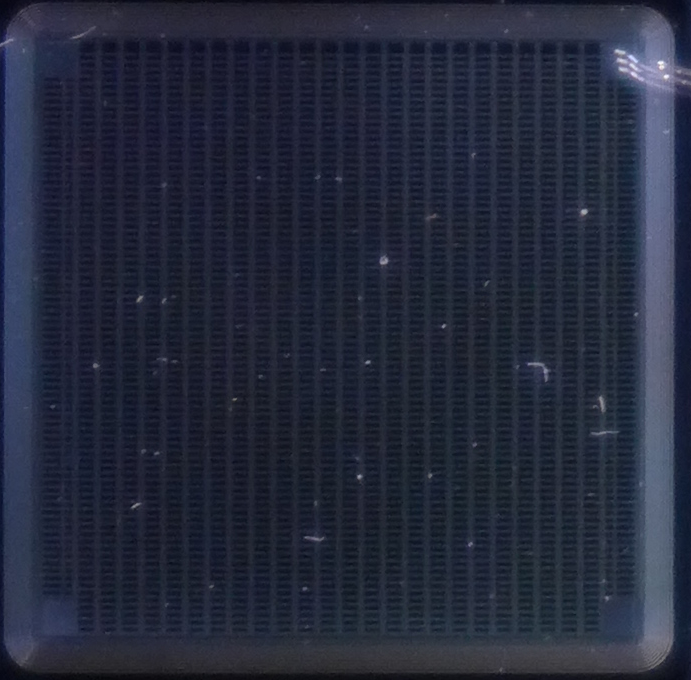
\includegraphics[height=3cm]{Pics/ROC0}
			\end{figure}
		\end{minipage}\no\s
	\end{center}
\end{frame}
% ============================
% THE SILICON PLANE
% ============================
\subsection{The Silicon Plane}
\begin{frame}
	\frametitle{The Silicon Plane}
	\begin{center}
		\begin{minipage}{4.5cm}
			\centering
			\begin{figure}
				\caption{analogue silcon plane}\vspace*{-5pt}
				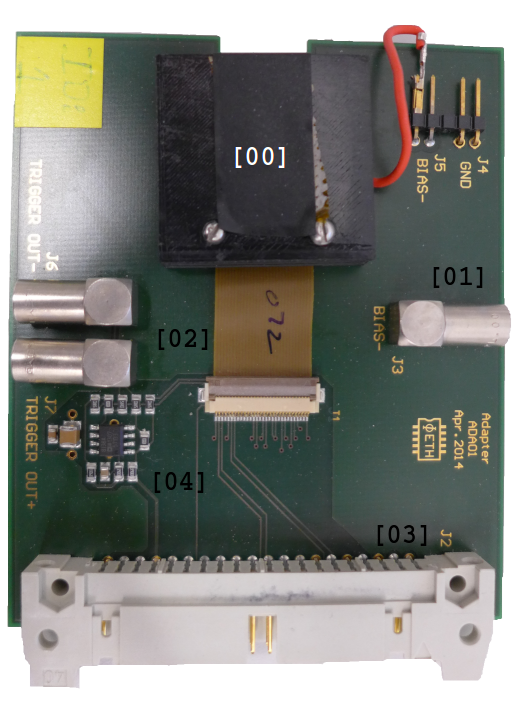
\includegraphics[width=4.2cm]{Pics/Plane}
			\end{figure}
		\end{minipage}
		\hspace*{2pt}
		\begin{minipage}{6cm}
			\begin{itemize}
				\item stable mounting framework for a single pixel detector [00]
				\item amplifying circuit [04]
				\item fast-OR differential LEMO output for pixel hits [02]
				\item no signal termination
				\item bias voltage LEMO connector for the sensors [01]
				\item 48 pin male connector on the back end [03]
			\end{itemize}
		\end{minipage}\no\s
	\end{center}
\end{frame}
% ============================
% THE OLD ANALOGUE TELESCOPE
% ============================
\subsection{The Analogue Telescope}
\begin{frame}
	\frametitle{The Analogue Telescope}
	\begin{itemize}
		\item main frame with six female 48 pin connectors for the planes [02]
		\item one male connector to a test-board (mainly built for an analogue test-board) [01]
		\item main operation mode: two planes in the front, two in the back to put a target in between
		\item two token jumper for the two empty connectors
		\item framework to hold the telescope and the target
	\end{itemize}
	\begin{center}
		\begin{minipage}{4cm}
			\centering
			\begin{figure}
				\caption{analogue telescope}
				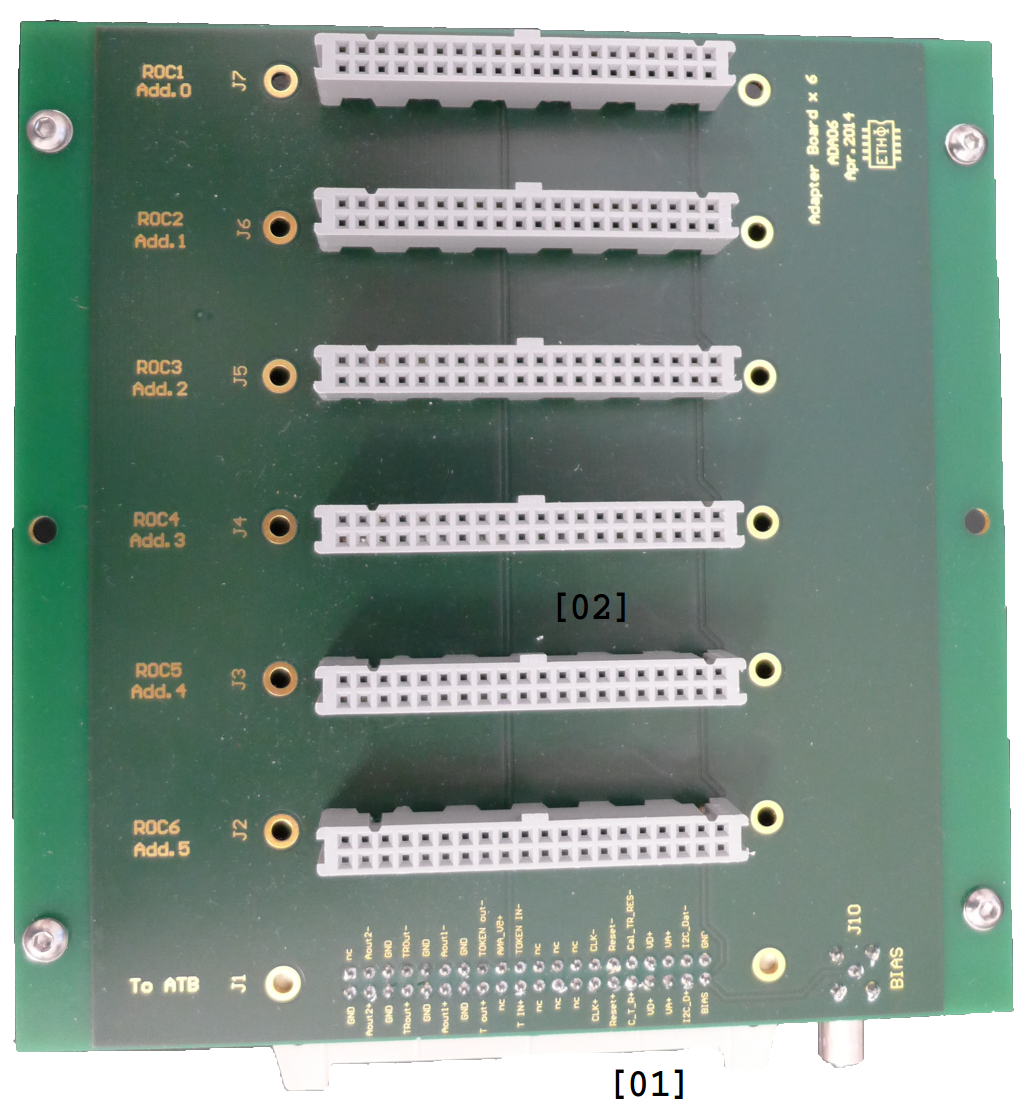
\includegraphics[height=3cm]{Pics/Telescope}
			\end{figure}
		\end{minipage}
		\hspace*{2pt}
		\begin{minipage}{2.5cm}
			\centering
			\begin{figure}
				\caption{jumper}
				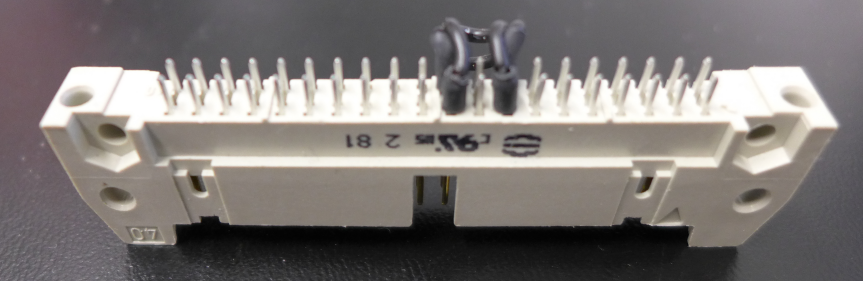
\includegraphics[width=2.5cm]{Pics/TokenJumper}
			\end{figure}
		\end{minipage}
		\hspace*{2pt}
		\begin{minipage}{4cm}
			\centering
			\begin{figure}
				\caption{mount for telescope}
				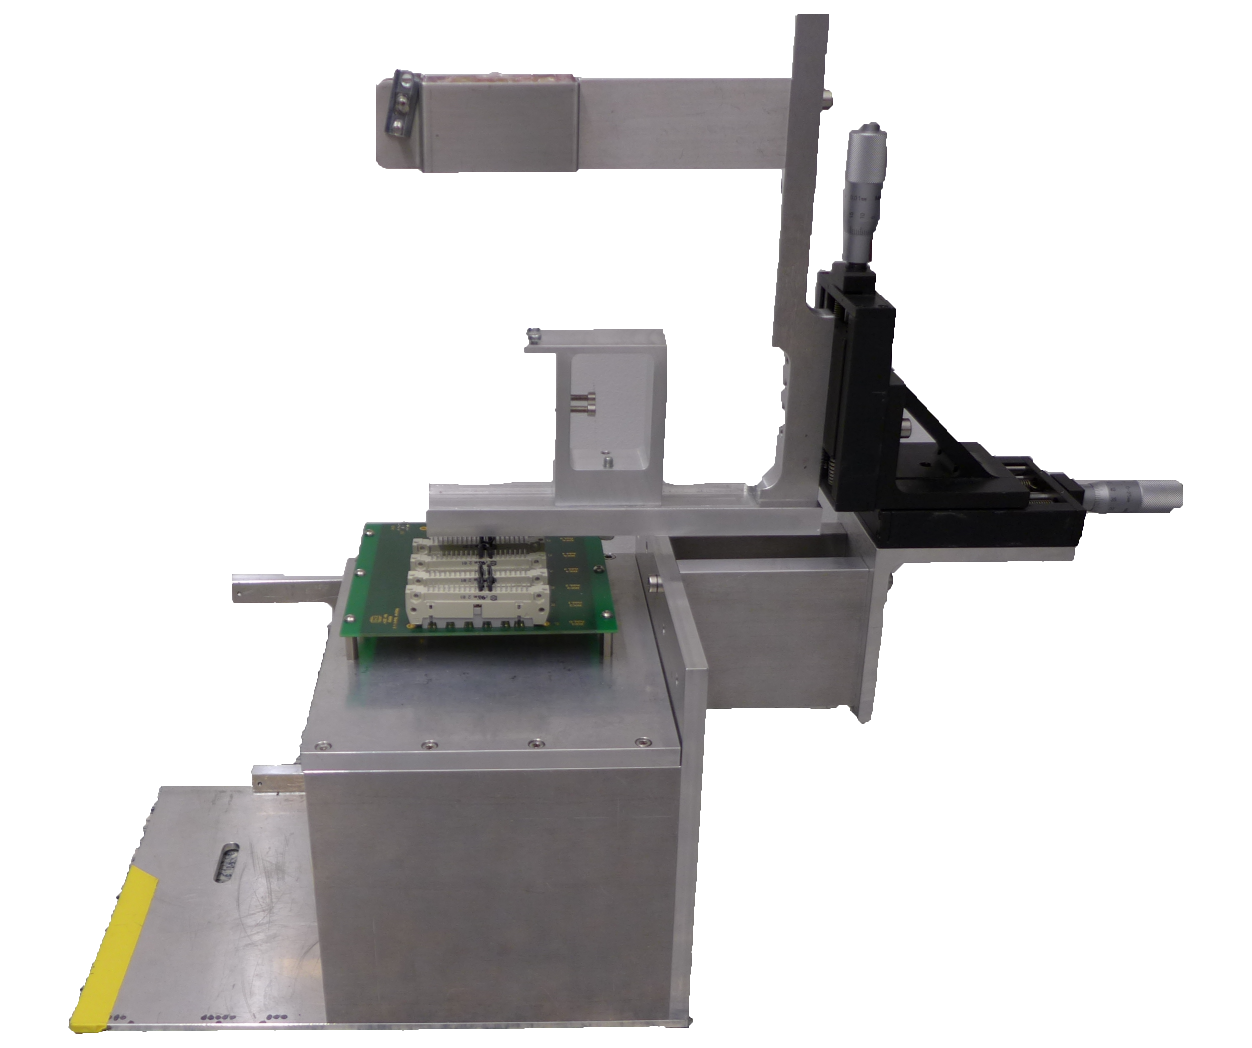
\includegraphics[width=3.5cm]{Pics/mounting}
			\end{figure}
		\end{minipage}\no\s
	\end{center}
\end{frame}
% ============================
% THE DIGITAL TESTBOARD
% ============================
\subsection{The Digital Test-Board (DTB)}
\begin{frame}
	\frametitle{The Digital Test-Board}
	\begin{itemize}
		\item FPGA including soft Token Bit Manager (TBM) emulator
		\item two digital and two analogue differential LEMO outputs which can be assigned to various internal signals
		\item clock and external trigger input
		\item connectors: USB, Ethernet, low voltage and  female scsi 
		\item LEMO hig voltage input 
	\end{itemize}
	\begin{center}
		\begin{minipage}{5cm}
			\centering
			\begin{figure}
				\caption{DTB top}
				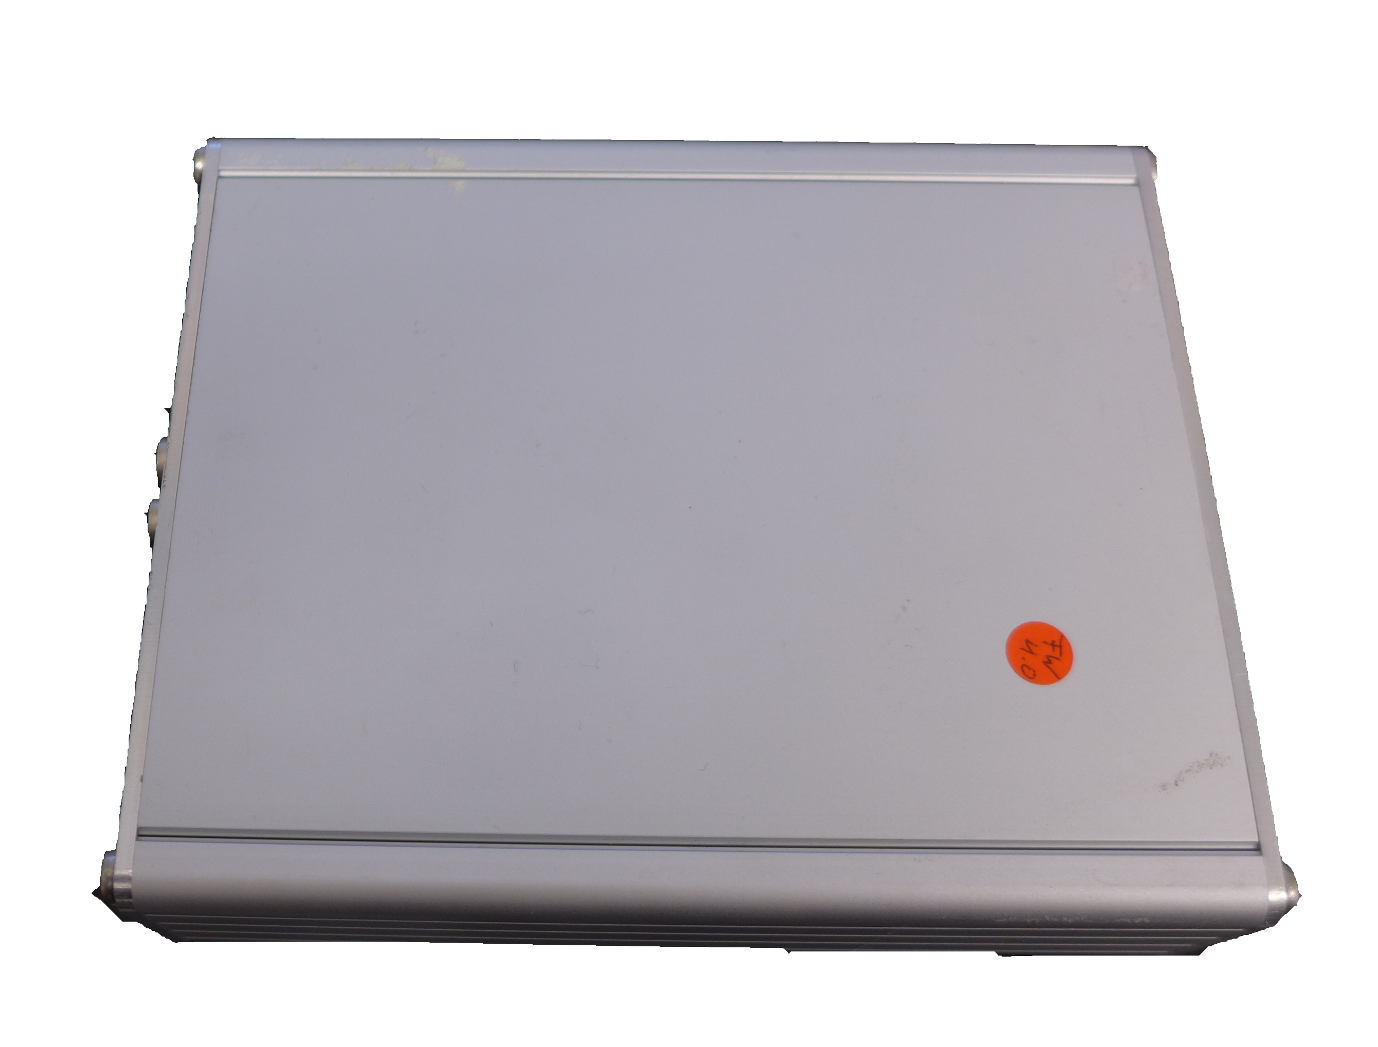
\includegraphics[width=4.5cm]{Pics/DTB}
			\end{figure}
		\end{minipage}
		\hspace*{2pt}
		\begin{minipage}{5cm}
			\centering
			\begin{figure}
				\caption{DTB front and back}
				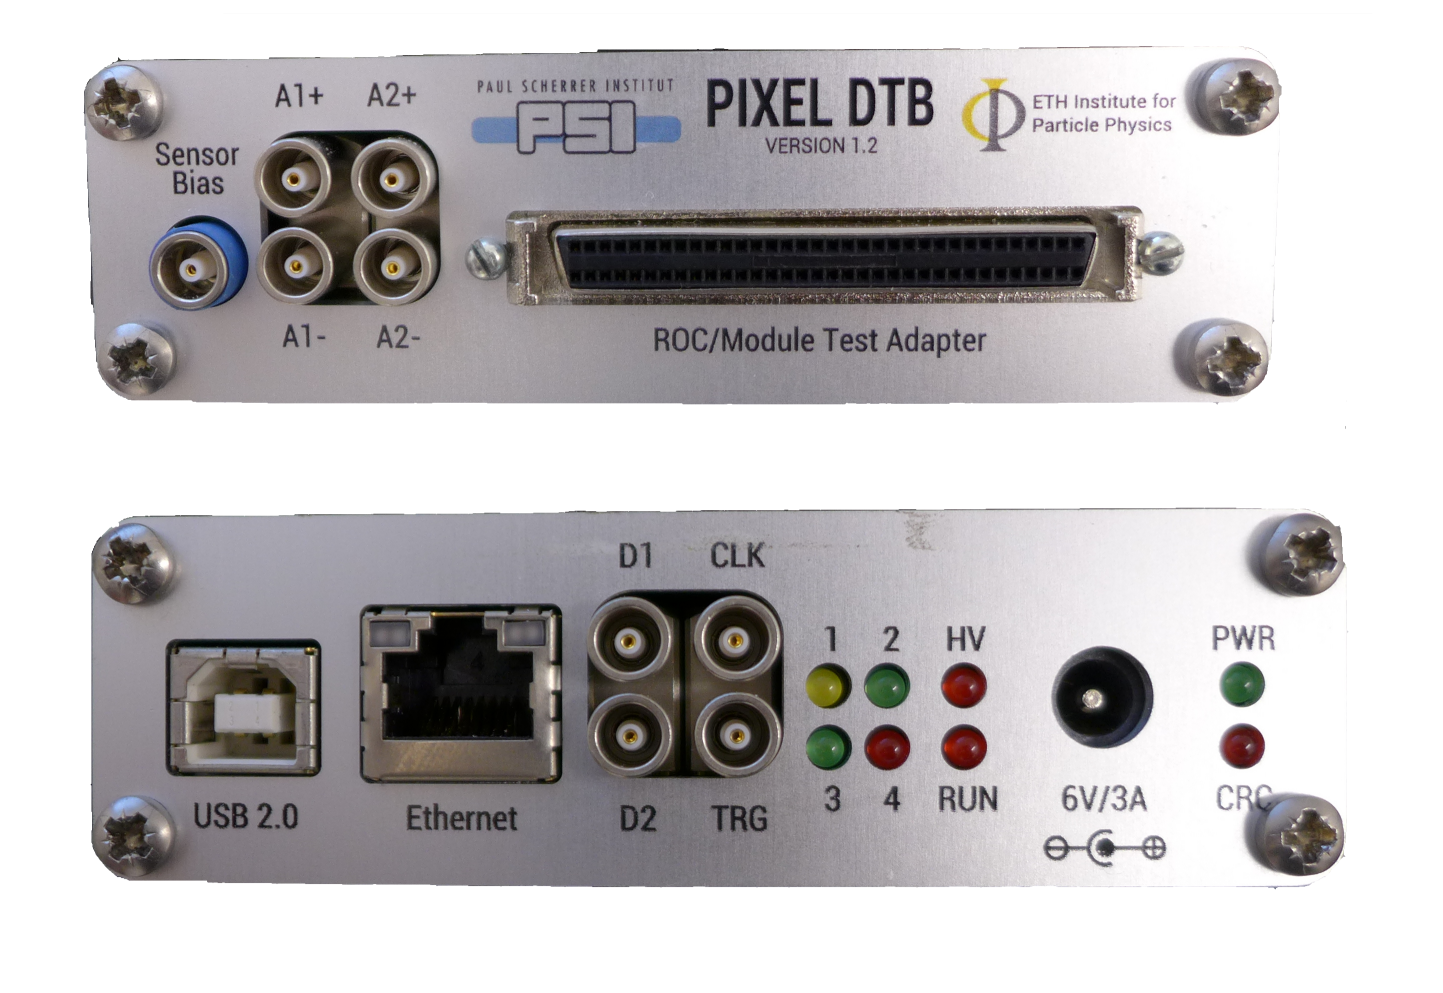
\includegraphics[width=4.5cm]{Pics/DTB-Sides}
			\end{figure}
		\end{minipage}\no\s
	\end{center}
\end{frame}

% % ============================
% % THE NEW TELESCOPE
% % ============================
% \subsection{The New Telescope}\begin{frame}TODO\end{frame}

% ====================================================================================
% SOFTWARE
% ====================================================================================
% \section{Software}
% \begin{frame}TODO\end{frame}
% \subsection{pXar}
% \subsection{Python Command Line Interface (CLI)}
% \subsection{EUDAQ}
% \subsection{Keithley Current}
% \subsection{EUDAQ Log Reader}
% \subsection{High Voltage Client}
% \subsection{Tracking}
% 
% ====================================================================================
% EXPERIMENTS AND MEASUREMENTS
% ====================================================================================
\section{Experiments \& Measurements}
% ============================
% DIGITAL READ OUT OF ANALOGUE PLANES
% ============================
\subsection{Digital Readout of the Analogue Planes}
\begin{frame}
	\frametitle{Digital Readout of the Analogue Planes}
	\begin{itemize}
		\item analogue planes built for readout with the Analogue Test Board (ATB)
		\item problem: limited buffer size thus limited amount of time for a single run
		\item idea: use pXar and the DTB for the readout
		\item pXar plug-in by Simon Spannagel can decode raw data from analogue ROC
		\begin{itemize}
			\item uses decoder according to the ROC type set in the configuration file\is
			\item all additional DAC parameters that are not used for the digital ROC appended to the pXar dictionary
		\end{itemize}
		\item analogue signal of the ROC converted by the ADC of the DTB
		\item additional timing settings for the DTB to determine the exact start and end point of the signal set in the test board configuration file
		\item goal: set the timing s.t. the first value is ultrablack and the last either the pulse height of the last pixel hit or the last DAC if no pixel was hit (or too many for that matter)
	\end{itemize}
\end{frame}
% new frame =========================================
\begin{frame}
	\frametitle{How to find the correct settings}
	\begin{itemize}
		\item connect the analogue ROC to the DTB (special adapter needed)
		\item start my pXar CLI with a set of working DAC parameters
		\begin{itemize}
			\item ./myscript -d \textit{\flq DAC directory\frq}
		\end{itemize}
		\item check if the ROC draws reasonable currents:
		\begin{itemize}
			\item getTBia\is
			\item getTBid
		\end{itemize}
		\item check weather the analogue current changes by changing the changing the analogue voltage
		\begin{itemize}
			\item setDAC vana \textit{\flq value\frq}
		\end{itemize}
		\item if the ROC is not responding i.e. the current is not changing $\rightarrow$ wrong sda settings
		\item inspect the outcome of a single activated pixel
		\begin{itemize}
			\item maskAllPixels 1 
			\item maskPixel 5 12 0
			\item daqStart
			\item daqTrigger \textit{\flq n\frq} 500
			\item daqGetRawEvent
			\item daqStop
		\end{itemize}
	\end{itemize}
\end{frame}
% new frame =========================================
\begin{frame}
	\frametitle{Analogue levels}
	\begin{center}
		\begin{minipage}{6cm}
			\begin{itemize}
				\item example output of the CLI with correct time settings: 
				\begin{itemize}
					\item \terminal{[-196, 0, 97, -54, 57, 106, 164, 212, 91]}
				\end{itemize}
				\item first three words: ROC header
				\begin{itemize}
					\item ultrablack, black, last DAC
				\end{itemize}
				\item next five words decoded pixel address
				\item last word: pulse height of the the pixel hit
				\item if there is only a header and no pixel information:
				\begin{itemize}
					\item no pixel or too many pixels activated
					\item wrong DAC vthreshcomp, caldel
					\item wrong delay of the calibrate pulse of the pattern generator
				\end{itemize}
			\end{itemize}
		\end{minipage}
		\hspace*{2pt}
		\begin{minipage}{4.5cm}
			\begin{figure}
				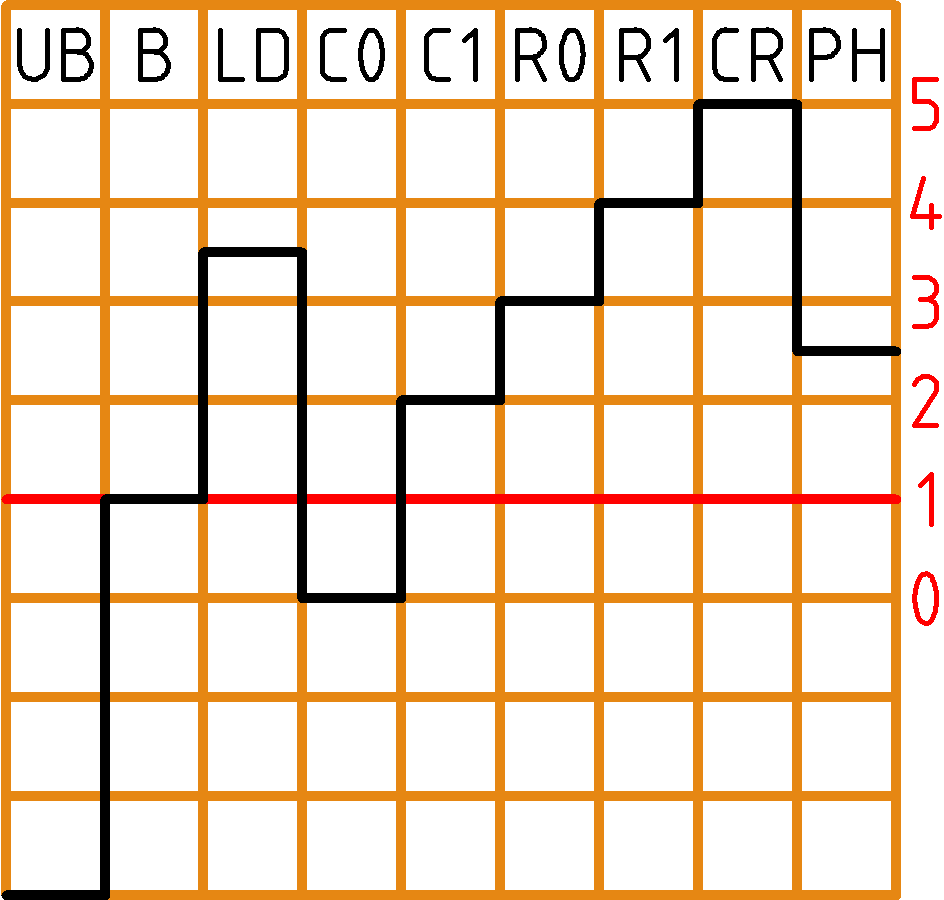
\includegraphics[width=4.5cm]{Pics/levels}
				\caption{example level scheme for pixel 5 12 }
			\end{figure}
		\end{minipage}\no\s
	\end{center}
\end{frame}
% new frame =========================================
\begin{frame}
	\frametitle{Adjusting the delays}
	\begin{center}
		\begin{minipage}{7cm}
			\begin{itemize}
				\item example output of the CLI with incorrect time settings: 
				\begin{itemize}
					\item \terminal{[-196, 0, 97, -54, 57, 106, 164, 212, 91]}
				\end{itemize}
				\item important delays:
				\begin{itemize}
					\item tindelay:  start sampling \plugin{n} clock cycles after sending the token in (tin)
					\item toutdelay: stop sampling \plugin{n} clock cycles after receiving the token out (tout)
				\end{itemize}
				\item implementing function \textit{\textcolor{red}{findAnalogueTBDelays}} for CLI to find the delays automatically:
				\begin{itemize}
					\item mask all pixels
					\item start with a low value for tindelay and increase it until the first word is lesser than $-100$ $\rightarrow$ ultrablack
					\item start with high value for toutdelay and decrease it until the last word is higher than $20$ $\rightarrow$ last DAC
					\item save and set the values
				\end{itemize}
			\end{itemize}
		\end{minipage}
		\hspace*{2pt}
		\begin{minipage}{3.5cm}
			\begin{figure}
				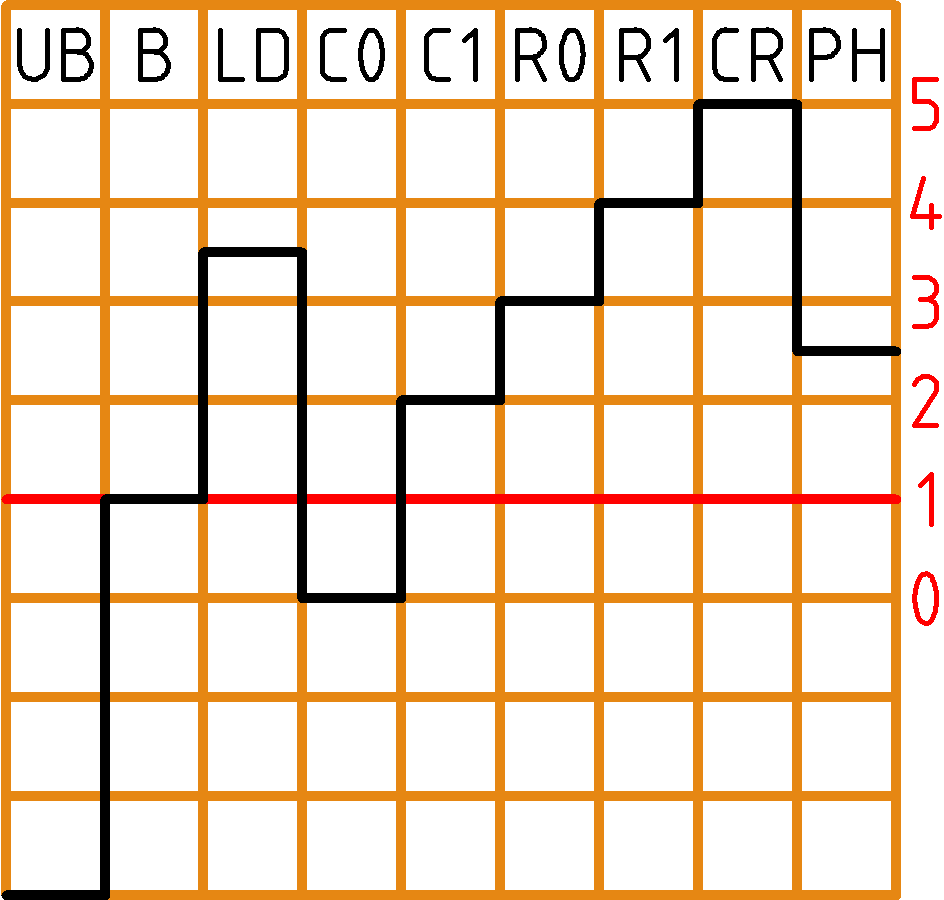
\includegraphics[width=3.2cm]{Pics/levels}
				\caption{output of findAnalogueTBDelays}
			\end{figure}
		\end{minipage}\no\s
	\end{center}
\end{frame}
% new frame =========================================
\begin{frame}
	\frametitle{Sampling point of the ADC}
	\begin{center}
		\begin{minipage}{5.5cm}
			\begin{itemize}
				\item analogue levels need some time within a clock cycle to reach the correct value
				\item need to adjust the clock phase (DTB delay in ns)
				\item sampling at the wrong phase will change the level depending on the previous or following one
			\end{itemize}
		\end{minipage}
		\hspace*{2pt}
		\begin{minipage}{5.2cm}
			\begin{figure}
				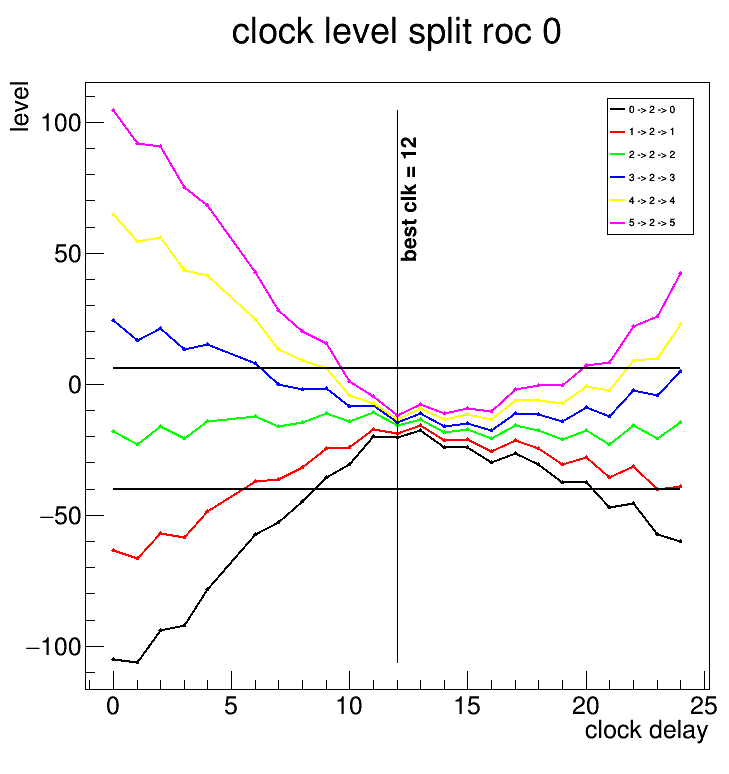
\includegraphics[width=4.9cm]{Pics/splits}
				\vspace*{-2pt}
				\caption{theoretical level split}
			\end{figure}
		\end{minipage}\no\s
	\end{center}
\end{frame}
% new frame =========================================
\begin{frame}
	\frametitle{Finding the clock delay}
	\begin{center}
		\begin{minipage}{5.5cm}
			\begin{itemize}
				\item activate six pixels where the levels go from $0\rightarrow$ fixed level $\rightarrow0$ \dots $5\rightarrow$ fixed level $\rightarrow5$
				\item activate the pixel 15/59 (1 1 1 1 1) to measure the black level
				\item black level important for decoding
				\item vary the clock phase from in between one cycle (0-24) 
				\item measure the values for the chosen fixed level
				\item calculate the averaged deviation from the mean value 
				\item choose the phase with minimal deviation
			\end{itemize}
		\end{minipage}
		\hspace*{2pt}
		\begin{minipage}{5.2cm}
			\begin{figure}
				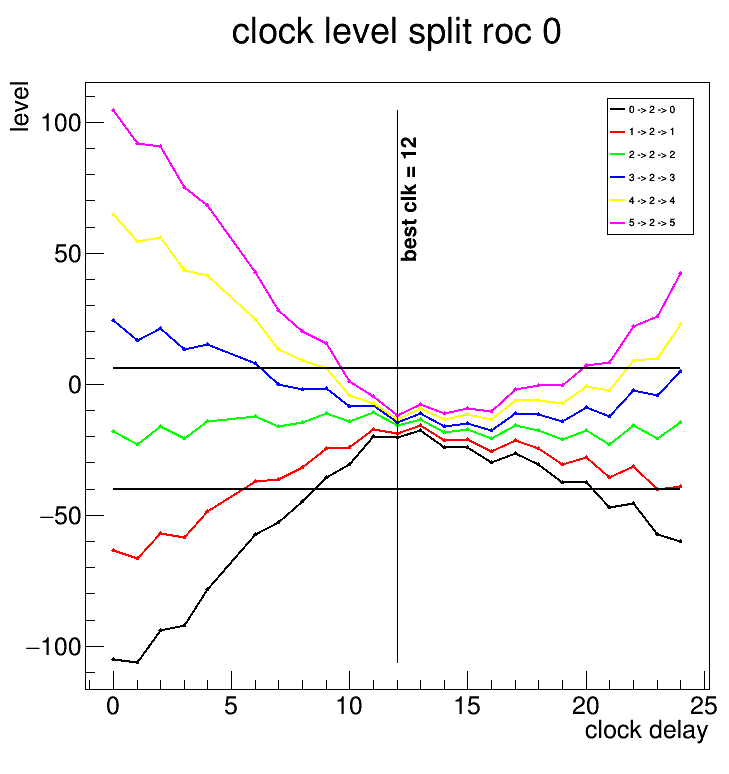
\includegraphics[width=4.9cm]{Pics/splits}
				\vspace*{-2pt}
				\caption{real level split}
			\end{figure}
		\end{minipage}\no\s
	\end{center}
\end{frame}
% new frame =========================================
\begin{frame}
	\begin{center}
		\begin{minipage}{5.5cm}
			\begin{itemize}
				\item might ended up in another clk cycle $\rightarrow$ run findAnalogueTBDelays again
				\item both telescopes slightly decrease the black level in the ROC header s.t. the decoding can go awry
				\item can be corrected either by adding the difference directly in the decoding
				\item or changing the DAC phscale
				\item implemented function to optimize for the black level spread
			\end{itemize}
		\end{minipage}
		\hspace*{2pt}
		\begin{minipage}{5.2cm}
			\begin{figure}
				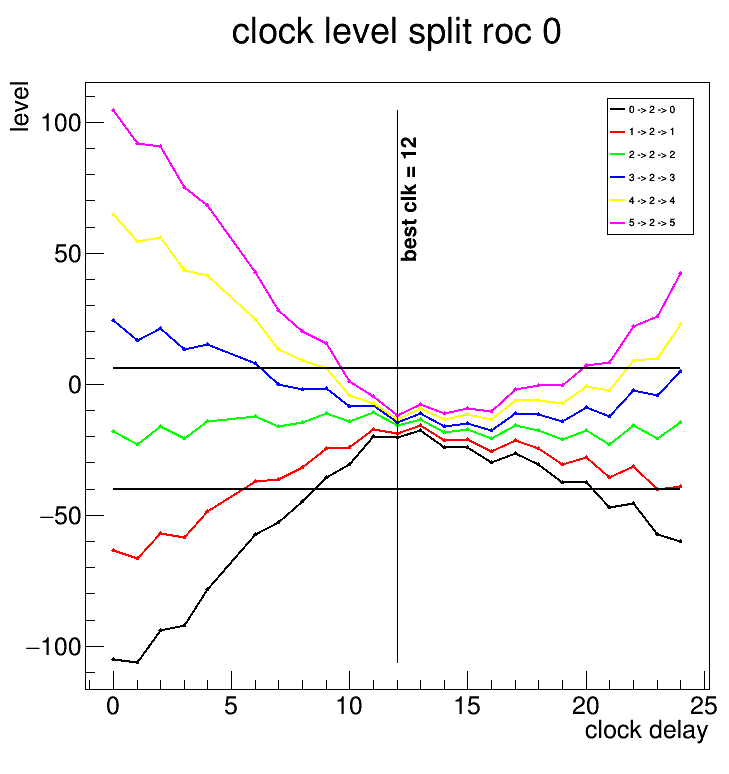
\includegraphics[width=4.9cm]{Pics/splits}
				\vspace*{-2pt}
				\caption{address levels}
			\end{figure}
		\end{minipage}\no\s
	\end{center}
\end{frame} 
% ============================
% TRACKING TELESCOPE
% ============================
\subsection{Tracking Telescope}
\begin{frame}
	\frametitle{Tracking Telescope}
	\begin{itemize}
		\item using n analogue planes of the PLT as tracking device
		\item analyse real data e.g. from the PSI test beam
		\item data acquired with the EUDAQ framework 
		\item requirement: root file converted with the DRS4 converter of EUDAQ
		\begin{itemize}
			\item \dots/\textit{eudaq-directory}/bin/Converter.exe -t drs4tree \textit{\flq binary data file \frq}
		\end{itemize}
		\item required branches: event\_number, time, plane, col, row, adc, charge
		\item using the the raw pixel data to align the planes, find tracks and put out some other useful information as follows
		\item adds the following branches to the root file:
		\begin{itemize}
			\item for tracking: slope\_x/y, chi2, chi2\_x/y, n\_tracks\is
			\item for track through the diamond: diam1/2\_track\_x/y, dist\_to\_dia1/2
			\item others: n\_tracks, charge\_all\_ROC1/\dots/n, hit\_plane\_bits
		\end{itemize}
		\item creates various plots %TODO add link where all the plots are shown
	\end{itemize}
\end{frame}
%==============
% \subsection{Study of the Fast-Or Signals}
% \subsection{DESY Test-Beam}
% \subsection{PSI Test-Beam}
% \begin{frame}TODO\end{frame}
% new frame =========================================
\begin{frame}
	\frametitle{}
	\begin{itemize}
		\item 
	\end{itemize}
\end{frame}
%==================================================================================================================================================
%===============================================SYNCHROTRON========================================================================================
%==================================================================================================================================================
% \section{Synchrotron}
% \subsection{Setup}
% \begin{frame}
% \begin{minipage}{4cm}
% \begin{center}
% % \includegraphics<1>[height=4cm]{Bilder/03}
% % \includegraphics<2>[height=4cm]{Bilder/04}
% % \includegraphics<3>[height=4cm]{Bilder/03}
% \end{center}
% \end{minipage}
% \hspace*{2pt}
% \begin{minipage}{6.5cm}
% \small\be\small F_R=F_L\ \rightarrow\ \frac{mv^2}{R}=qvB\ee
% \be \curvearrowright\ p=mv=qBR\ee
% \be \uptau=\frac{2\uppi R}{v}\ka \curvearrowright\ka \upomega_c=\frac{v}{R}=\frac{qB}{m_e\upgamma}\ee
% \begin{center}
% $\upomega_c-\z{cyclotron frequency}$
% \end{center}
% \end{minipage}\no\s
% \begin{overprint}
% \onslide<1>
% \bi \small
% 	\item constant radius $R$ and increasing magnetic Field $B$
% \ei
% \onslide<2>
% \bi \small
% 	\item constant radius $R$ and increasing magnetic Field $B$
% 	\item done with one or more preaccelerators: Cockroft-Walton $\rightarrow$ linac $\rightarrow$ pre-synchrotron $\rightarrow$ real synchrotron
% 	\bi	\item neccessary amount of energy to keep particles on a fixed circular orbit
% 		\item ratio of injected to maximum energy has to be small $\rightarrow$ higher acceptance $\curvearrowright$ gain in intensity\ei
% 	\item first accelerator called booster, last called main ring
% \ei
% \onslide<3>
% \bi\small
% 	\item magnets that keep particles on circular trajectory (bending magnets): dipole magnets
% 	\item focussing magnets: quadrupole magnets
% 	\item accelerating tube: radio frequency (RF) cavity
% 	\item synchronized frequency so that acceleration every time passing a cavity
% 	\item no continous beam $\rightarrow$ bunching in a linac ($\sim 1\,$mm bunch size)
% \ei 
% \end{overprint}
% \end{frame}
%==================================================================================================================================================
%===============================================SYNCHROTRON========================================================================================
%==================================================================================================================================================
% \subsection{Beam stability}
% \begin{frame}
% \frametitle{Beam stability}
% \bi
% 	\item velocity dispersion of the particles in the bunch
% 	\item Synchrotron can work if the not exactly synchronous particles 
% 	\bi \item tend to converge \item oscillate around the center \ei
% 	\item no stable acceleration if motion diverges
% \ei
% \end{frame}
% %==================================================================================================================================================
% %===============================================BETATRON OSCILLATION===============================================================================
% %==================================================================================================================================================
% \begin{frame}
% \frametitle{a) Betatron oscillation}
% \begin{minipage}{5.5cm}
% \begin{center}
% \includegraphics[width=4cm]{Bilder/13}
% \end{center}
% \end{minipage}
% \hspace*{2pt}
% \begin{minipage}{5.5cm}
% \begin{center}
% \includegraphics[width=4cm]{Bilder/14}
% \end{center}
% \end{minipage}\no\s
% \bi \small
% 	\item oscillations transverse to the beam
% 	\item controlled by quadrupole magnets
% 	\item one quadrupole: focussing only in one transverse direction, defocussing in the other
% 	\item two quadropoles (one turned by 90�): focussing in both directions\as
% 	\item $\rightarrow$ Synchrotron: interchanging dipole and quadrupole magnets in a FDFDFD... structure
% \ei
% \end{frame}
% %==================================================================================================================================================
% %===============================================PHASE STABILITY====================================================================================
% %==================================================================================================================================================
% \begin{frame}
% \frametitle{b) Phase stability}
% \begin{minipage}{4cm}
% \begin{center}
% \includegraphics[width=4cm]{Bilder/05}
% \end{center}
% \end{minipage}
% \hspace*{2pt}
% \begin{minipage}{7.5cm}
% \bi \small
% 	\item longitudinal oscillation synchronized with applied RF-voltage: synchrotron oscillation
% 	\item circular motion of $O$ is synchronous with RF (always the same acceleration) $\rightarrow$ synchronous phase
% \ei
% \end{minipage}\no\s
% \bi \small
% 	\item too early arriving particle $E$: 
% 	\bi \item gets more acceleration (more $E$) $\rightarrow$ more effective mass $\curvearrowright$ with $v\approx c$ bigger Radius
% 		\item $\uptau=\frac{R}{v}$ increases $\rightarrow$ arrive later next turn at $E'$\ei
% 	\item too late arriving particle $L$ gets less $E$ $\rightarrow$ smaller Radius $\rightarrow$ arrive earlier at $L'$
% \ei
% $\rightarrow$ convergation to synchronous phase
% 
% 
% \end{frame}
% %==================================================================================================================================================
% %===============================================RESULTS============================================================================================
% %==================================================================================================================================================
% \subsection{Synchrotron radiation}
% \begin{frame}
% \frametitle{Synchrotron radiation}
% \bi 
% 	%\item attenuates both betatron and sychrotron oscillation $\rightarrow$ also stabilizes the beam
% 	\item particle emits light when a electromagnetic field exerts a force on it (e.g. bended by a magnet)
% 	\item energy cannot be made arbitrary large proportional to the radius
% 	\item energy loss too large to be compensated
% 	\be \Updelta E=\frac{4\uppi\hbar c \upbeta^3\upgamma^4}{3R}\ee
% 	\be \Updelta E[\z{MeV}] \sim \frac{0.0085(E[\z{GeV}])^2}{R[\z{m}]}\ka \z{for electrons}\ee
% 	\item at LEP: $\Updelta E=3.2\,$GeV/turn ($R=2804\,$m $E=100\,$GeV)
% 	\item proton is 2000 times heavier $\curvearrowright$ loss is $2000^4\sim 10^{13}$ times smaller 
% 	\item $\Updelta E=6.7\,$keV/turn at LHC
% \ei
% \end{frame}
% %==================================================================================================================================================
% %===============================================APPLICATIONS=======================================================================================
% %==================================================================================================================================================
% \subsection{Applications}
% \begin{frame}
% \begin{minipage}{5.5cm}
% X-ray microscopy
% \end{minipage}
% \hspace*{2pt}
% \begin{minipage}{5cm}
% \begin{center}
% \includegraphics[width=5cm]{Bilder/15}
% \end{center}
% \end{minipage}\no\s
% \begin{minipage}{5.5cm}
% determine the origin of chrystals
% \bi  \item origin of blood diamonds \ei
% \end{minipage}
% \hspace*{2pt}
% \begin{minipage}{5cm}
% \begin{center}
% \includegraphics[width=5cm]{Bilder/16}
% \end{center}
% \end{minipage}\no\s
% \end{frame}
% %==================================================================================================================================================
% %===============================================APPLICATIONS=======================================================================================
% %==================================================================================================================================================
% \begin{frame}
% \begin{minipage}{5.5cm}
% Micromachining 
% \bi \item production of tiny machine parts  \ei
% \end{minipage}
% \hspace*{2pt}
% \begin{minipage}{5cm}
% \begin{center}
% \includegraphics[width=5cm]{Bilder/17}
% \end{center}
% \end{minipage}\no\s
% \begin{minipage}{5.5cm}
% Medicine and Pharmaceuticals
% \bi\item study and model influenza virus proteins \ei
% \end{minipage}
% \hspace*{2pt}
% \begin{minipage}{5cm}
% \begin{center}
% \includegraphics[width=5cm]{Bilder/18}
% \end{center}
% \end{minipage}\no\s
% \end{frame}
% %==================================================================================================================================================
% %===============================================XFEL=========================================================================================
% %==================================================================================================================================================
% \section{Free Electron Laser}
% \subsection{Setup}
% \begin{frame}
% \bi 
% 	\item emittance of synchrotron radiation (SR) if electromagnetic fields exerts force on a charged particle
% 	\item use external electromagnetic fields to emit even more SR
% 	\item particle continously has to lose energy into SR $\rightarrow$ field must have certain frequency and phase
% \ei
% \pause
% \begin{center}
% \includegraphics[height=2.5cm]{Bilder/07}
% \end{center}
% \bi 
% 	\item generally: recycling and usage of spontaneous radiation for next emissions by using mirrors
% 	\item lack of suitable mirros in UV and X-Ray regimes
% \ei
% \end{frame}
% \begin{frame}
% SwissFEL facility with beam line tunnel experimental hall and infrastructure
% \begin{center}
% \includegraphics[width=12cm]{Bilder/06}
% \end{center}
% \end{frame}
% 
% %==================================================================================================================================================
% %===============================================WORKING PRINCIPLE I================================================================================
% %==================================================================================================================================================
% \subsection{Working principle}
% \begin{frame}
% \bi 
% 	\item propagation on a sinusoidal path with $v\simeq c$
% 	\item emittance of SR in a small cone in forward direction
% 	\item radiation from individual magnetic periods overlap $\rightarrow$ interference
% \ei
% \begin{center}
% \includegraphics[width=6cm]{Bilder/08}
% \end{center}
% \bi 
% 	\item SR faster then the electron
% 	\item electrons have to slip one radiation wavelength with respect to the faster electromagnetic field during one period of the undulator
% 	%\item $\curvearrowright$ amplification
% \ei
% \end{frame}
% 
% %==================================================================================================================================================
% %===============================================WORKING PRINCIPLE II===============================================================================
% %==================================================================================================================================================
% \begin{frame}
% \begin{center}
% \includegraphics[width=12cm]{Bilder/09}
% \end{center}
% \bi \small
% 	\item Interaction of the oscillating bunge and the electromagnetic field
% 	\item deceleration if electron and e/m-wave are in phase
% 	\item acceleration if off phase
% 	\item longitudinal fine structure called microbunching
% 	\item longitudinal distribution cut into equidistant slices
% 	%\item seperation length: wavelength of the emitted radiation
% 	\item more and more electrons start radiating in phase
% 	\item incresingly coherent superposition of the radiation 
% 	\item extremely short and intense X-ray flashes with the properties of laser light
% \ei
% \end{frame}
% %==================================================================================================================================================
% %===============================================APPLICATIONS I=====================================================================================
% %==================================================================================================================================================
% \subsection{Applications}
% \begin{frame}
% \frametitle{Deciphering the structure of biomelocules}
% \bi \item X-ray sources not strong enough to look at single molecules\ei
% \begin{center}
% \includegraphics[width=7cm]{Bilder/10}
% \end{center}
% \end{frame}
% %==================================================================================================================================================
% %===============================================APPLICATIONS II====================================================================================
% %==================================================================================================================================================
% \begin{frame}
% \frametitle{Filming chemical reactions}
% \bi \item flashes: less than 0.1 trillionth of a second $\rightarrow$ snapshots without moving details becoming blurred\ei
% \begin{center}
% \includegraphics[width=7cm]{Bilder/11}
% \end{center}
% \end{frame}
% %==================================================================================================================================================
% %===============================================APPLICATIONS III===================================================================================
% %==================================================================================================================================================
% \begin{frame}
% \frametitle{Investigate extreme states of matter}
% \bi \item plasmas can be created that are as hot as the interiors of giant stars\ei
% \begin{center}
% \includegraphics[width=7cm]{Bilder/12}
% \end{center}
% \end{frame}



\end{document}